\chapter{Populäre Cross-Plattform Frameworks}
\label{ch:Frameworks}

Im Folgenden sollen die vier populärsten Frameworks für die Cross-Plattform Entwicklung näher betrachtet werden.
Dabei liegt der Fokus auf der Funktionsweise der Frameworks, der Einordnung in eine der Kategorien nach Nunkesser und eine kurze Bewertung der zu erwartenden Performance basierend auf existierenden Untersuchungen.

Zur Identifikation der populärsten Frameworks werden insbesondere die Stack Overflow Developer Surveys der letzten zwei Jahre \cite{Stackoverflow_2021} \cite{Stackoverflow_2022} herangezogen, welche Entwickler unter anderem zu ihren bevorzugten und im professionellen Bereich eingesetzten Frameworks befragen.
Aus diesen Frameworks werden diejenigen ausgewählt, die in die Kategorie Cross-Plattform fallen.
Daneben kommen die Daten von Appfigures zu den am häufigsten in den App-Stores vertretenen Frameworks \cite{Appfigures_TopSDKs} zum Einsatz.
Weiterhin wird auf die Umfrage \cite{Statista_UsedCrossPlatformFrameworks} zurückgegriffen, welche die am häufigsten eingesetzten Cross-Plattfom Frameworks zwischen 2019 und 2021 ermittelt hat.
In dieser Umfrage gab etwa ein Drittel der befragten Entwickler im Bereich der mobilen App-Entwicklung an, ein Cross-Plattform Framework zu verwenden.
Im Jahr 2021 verwendeten 42 \% von diesen Entwicklern Flutter, was es zum am häufigsten genutzten Framework macht.
ReactNative kommt in dieser Umfrage auf 38 \%, Cordova auf 16 \% und Ionic ebenfalls auf 16 \%
Das Problem hierbei ist, dass Ionic kein Cross-Plattform Framework ist, sondern selbst auf die Cross-Plattform Frameworks Cordova oder Capacitor aufsetzt \cite{Ionic_Docs}.
Deshalb müssen Ionic und Cordova zusammengefasst und dementsprechend gemeinsam betrachtet werden.
Das am vierthäufigsten eingesetzte Framework ist damit Xamarin mit 11 \% \cite{Statista_UsedCrossPlatformFrameworks}.

In der Stack Overflow Developer Survey von 2021 \cite{Stackoverflow_2021} sind nur React Native(16,48 \%), Flutter (13,35 \%) und Cordova (8,67 \%) als Cross-Plattform Frameworks erwähnt.
Da diese Umfrage sich nicht nur auf Entwickler mobiler Anwendungen fokussiert, sind hier die Anteile der eingesetzten Frameworks deutlich kleiner.
2022 sind in der Stack Overflow Developer Survey \cite{Stackoverflow_2022} Flutter (13,62 \%), React Native(12,56 \%), Ionic (5,97 \%) und Xamarin (5,54 \%), die vier am häufigsten eingesetzten Frameworks.

\begin{figure}[ht]
  \centering
  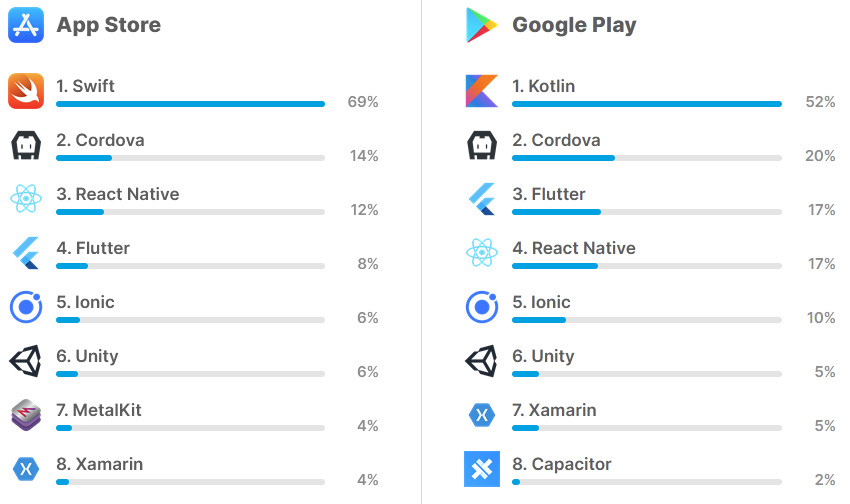
\includegraphics[width=0.8\textwidth]{top_sdks}
  \caption{Die am häufigsten in den App-Stores vertretenen \acp{SDK} \cite{Appfigures_TopSDKs}.}
  \label{fig:top_sdks}  
\end{figure}

\autoref{fig:top_sdks} zeigt die \acp{SDK}, welche in den jeweiligen App-Stores am meisten zum Einsatz kommen.
Neben Cross-Plattform Frameworks, sind hier auch die nativen \acp{SDK} aufgeführt.
Laut Appfigures \cite{Appfigures_TopSDKs} ist Cordova sowohl in Apples App-Store als auch im Google Play-Store das am häufigsten verwendete Framework.
Danach folgen in beiden App-Stores React Native, Flutter und Ionic in leicht unterschiedlicher Reihenfolge.
Auch hier gilt, dass Ionic nicht als eigenständiges Frameworks angesehen werden kann, sondern nur in Verbindung von Cordova oder Capacitor betrachtet werden kann.
Demnach wäre Unity das am vierthäufigsten eingesetzte Framework.
Aufgrund des starken Fokus auf Spieleentwicklung \cite{Unity} wird Unity in dieser Arbeit allerdings nicht als typisches Cross-Plattform Framework angesehen.
Den nächsten Platz belegt auch in den Daten von Appfigures Xamarin.

Damit kommen alle herangezogenen Daten zu den am häufigsten eingesetzten Frameworks zu dem Ergebnis, dass Flutter, React Native, Cordova und Xamarin die vier populärsten Frameworks sind.
Da der Einsatz von Ionic weit verbreitet ist, wird auch kurz auf Ionic in Kombination mit Cordova eingegangen.

\section{Flutter}
\label{sec:Frameworks_Flutter}

Das Framework Flutter wird primär von Google entwickelt und ist unter der permissiven BSD-Lizenz verfügbar.
Die erste Beta-Version wurde 2018 veröffentlicht \cite{Sharma_Flutter}.
Flutter setzt einen starken Fokus auf das \ac{UI} mobiler Anwendungen und zielt darauf ab, das \ac{UI} an den Stil der jeweiligen Plattform anzupassen \cite{Flutter_Architektur}.


Die Basis von Flutter bildet die, ebenfalls von Google entwickelte, Programmiersprache Dart.
Dart ist darauf ausgelegt, eine Vielzahl von Plattformen direkt zu unterstützen, wie in \autoref{fig:dart_build} dargestellt.
Das Flutter-Framework unterstützt die gleichen Plattformen wie Dart und erlaubt somit die Entwicklung für Android, iOS, Windows, macOS und das Web.
\begin{figure}[ht]
    \centering
    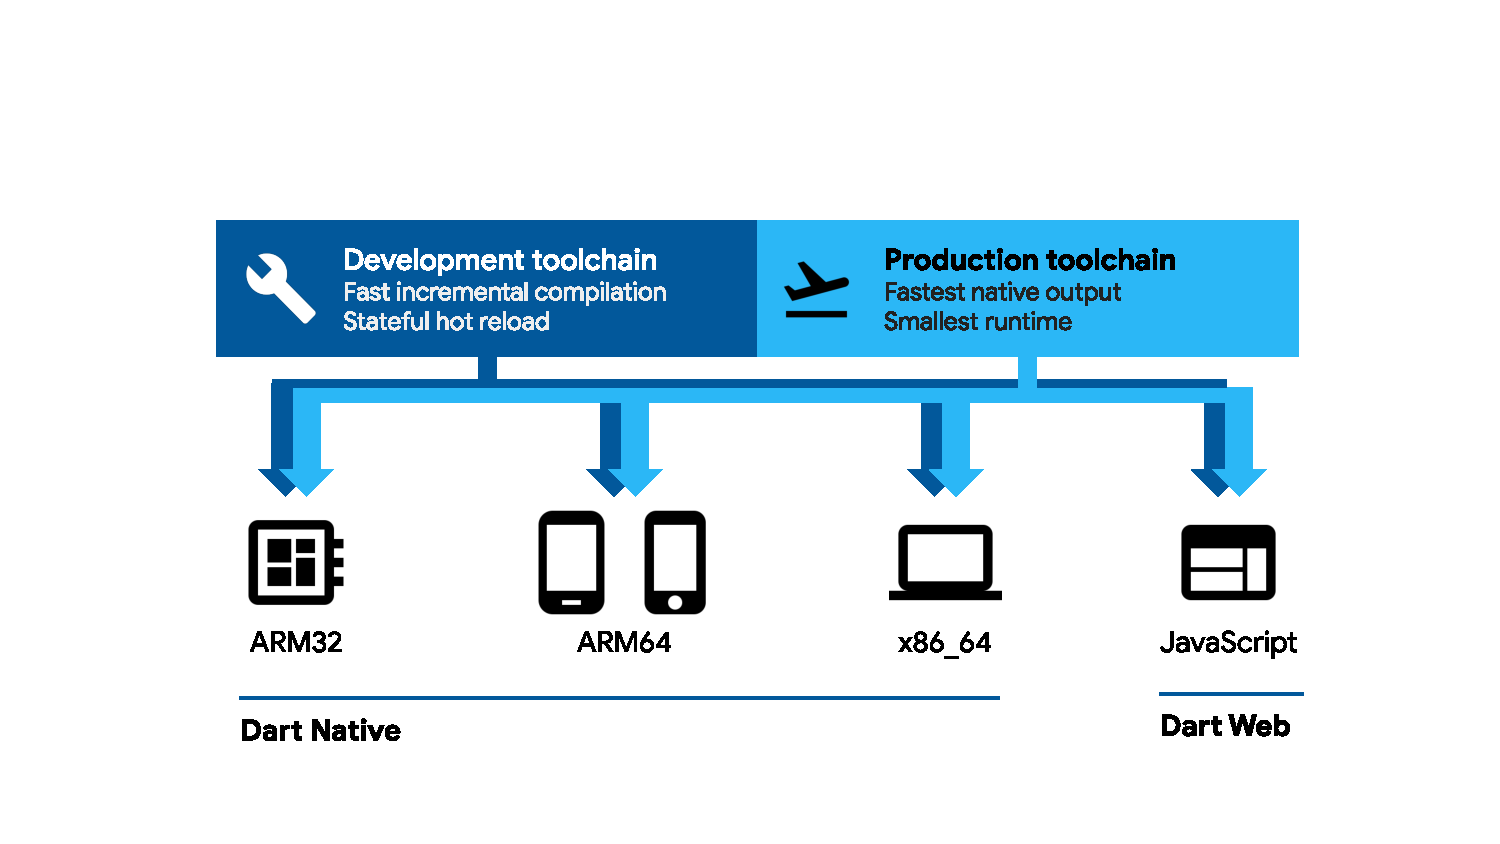
\includegraphics[clip, trim=2.5cm 1cm 0 2cm, width=1.1\textwidth]{dart_build.pdf}
    \caption{Zielplattformen von Dart/Flutter \cite{Dart_Overview}}
    \label{fig:dart_build}
\end{figure}


Dart unterstützt für die native Kompilierung mit \textit{Dart Native} die Verwendung eines \ac{AOT}- oder eines \ac{JIT}-Compilers.
Für \textit{Dart Web} wird der Dart-Code in JavaScript transpiliert und kann somit in Webbrowsern interpretiert werden \cite{Flutter_Architektur}.
Der \ac{JIT}-Compiler ist Teil der \textit{Development toolchain} und wird vor allem während der Entwicklung verwendet um die Build-Zeiten kurz zu halten.
Für die Auslieferung einer in Dart geschriebenen Anwendung wird üblicherweise der \ac{AOT}-Compiler der \textit{Production toolchain} verwendet.
Durch direkte Kompilation in Plattformspezifischen Assembler-Code und zusätzliche Optimierungen werden so im Allgemeinen performantere Anwendungen erzeugt.
Der Wegfall der \ac{JIT}-Kompilierung beim Anwendungsstart sorgt außerdem für schnelle Startzeiten \cite{Dart_Overview}.



Flutter verwendet für die nativen Plattformen eine dreischichtige Architektur.
Wie in \autoref{fig:flutter_architecture} gezeigt, besteht diese aus den Schichten \textit{Framework}, \textit{Engine} und \textit{Embedder}.
Die eigentliche Anwendung wird über der Framework-Schicht umgesetzt und kann die Abstraktionen der darunterliegenden Schicht verwenden.
\begin{figure}[h]
    \centering
    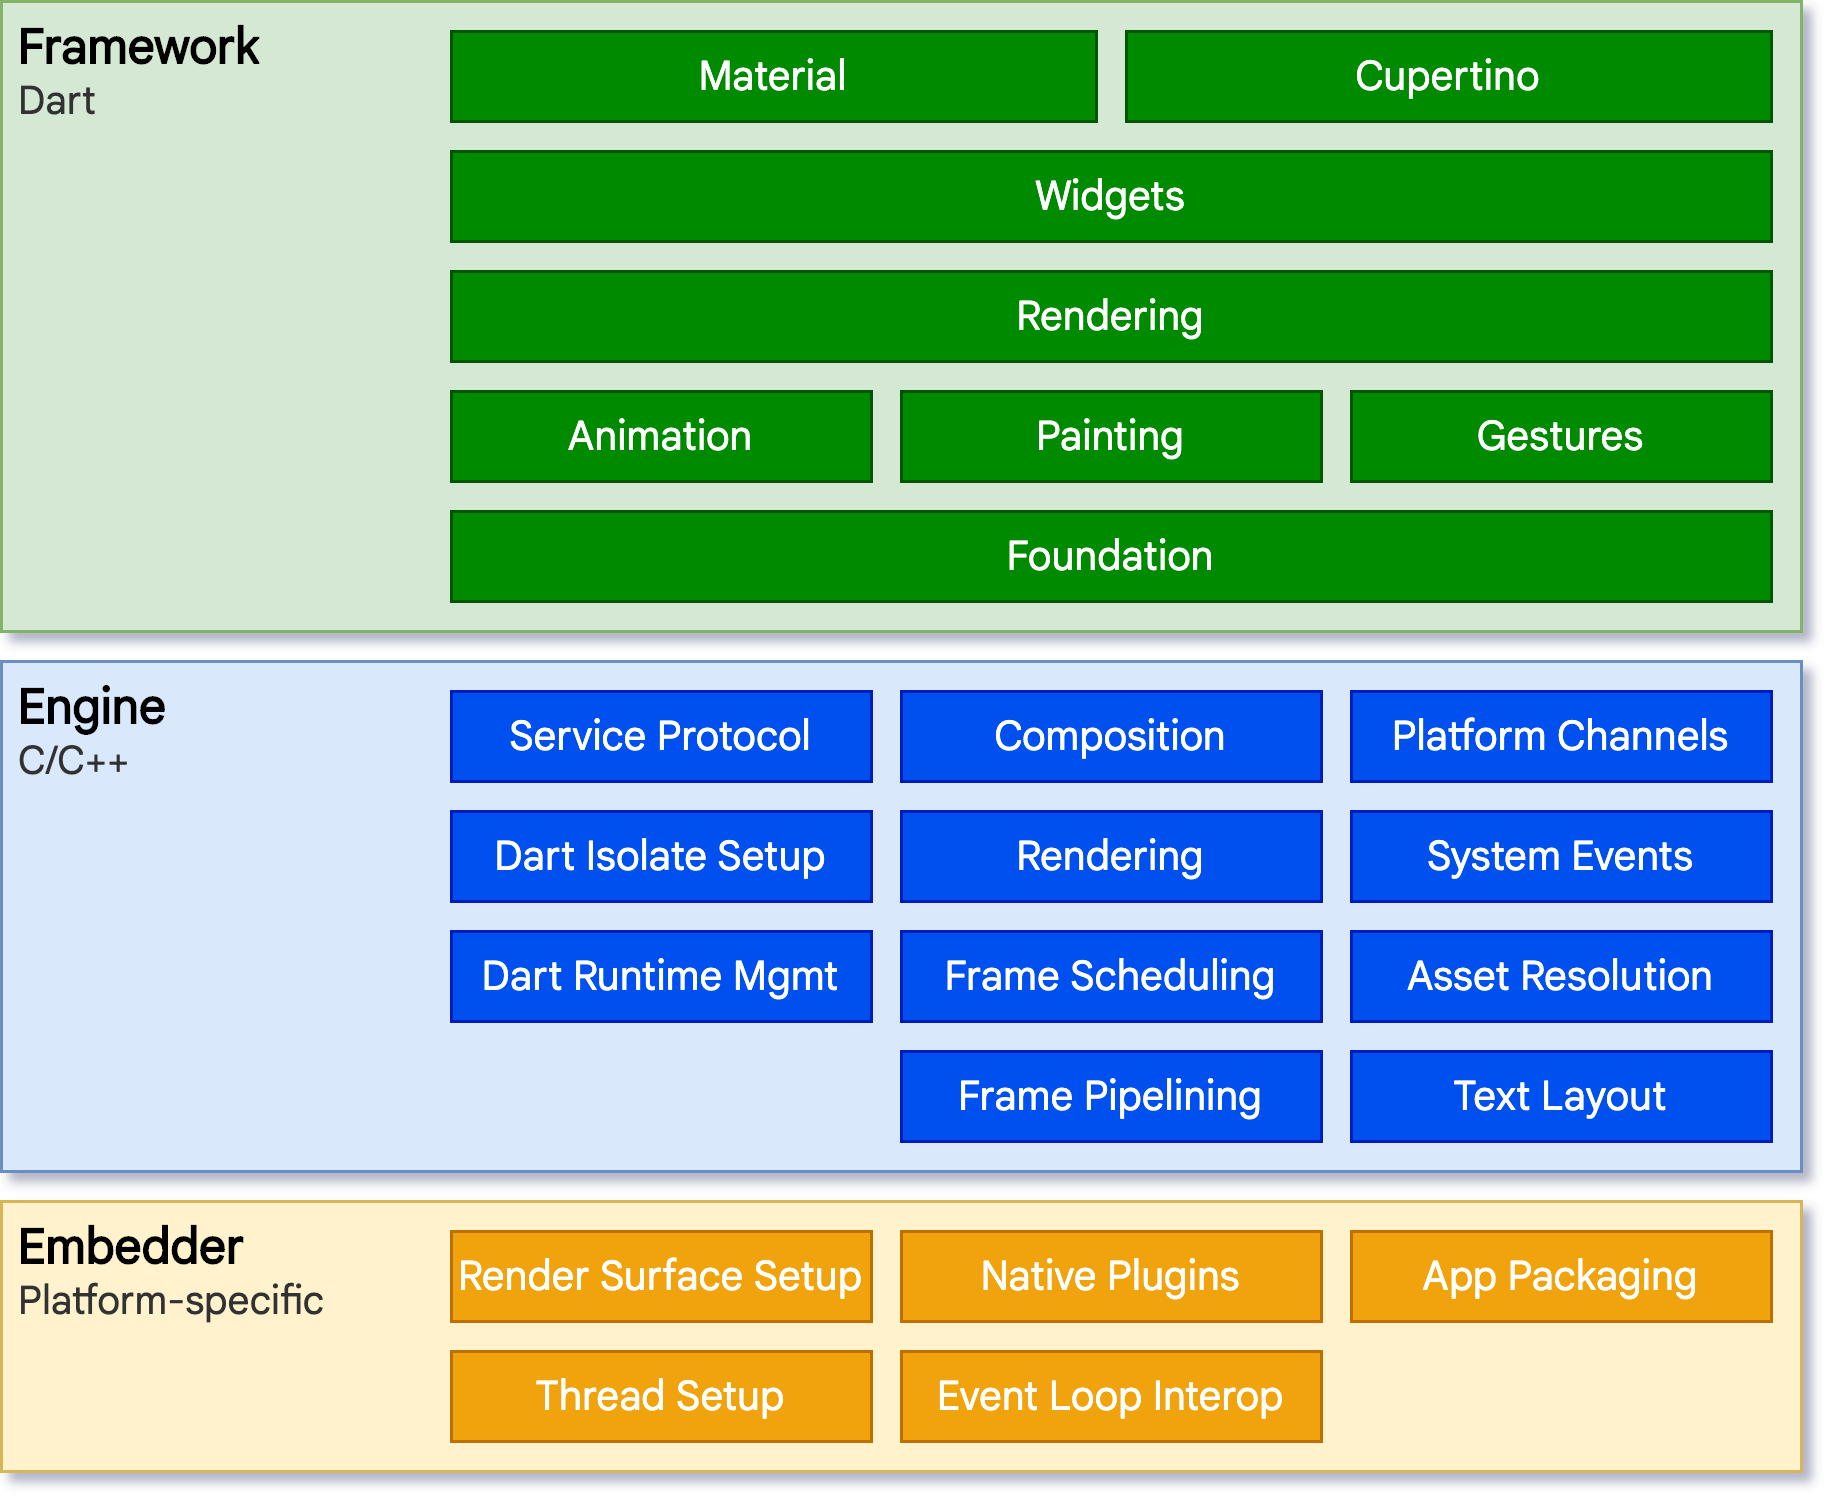
\includegraphics[width=0.9\textwidth]{flutter_architecture.png}
    \caption{Schichtenarchitektur des Flutter-Frameworks \cite{Flutter_Architektur}}
    \label{fig:flutter_architecture}
\end{figure}

Die Basis bildet die Embedder-Schicht, welche als einzige plattformspezifisch ist und der darüber liegenden Schicht eine einheitliche Schnittstelle zum unterlagerten System zur Verfügung stellt.
Für die verbreiteten Plattformen, wie Android und iOS, steht eine Standard-Implementierung bereit.
Zusätzlich können jedoch auch eigene Embedder implementiert werden, um weitere Plattformen zu unterstützen \cite{Flutter_Architektur}.

Auf den Embedder setzt die Flutter-Engine auf, welche die Flutter-\acp{API} bereitstellt und das Rendering der Oberfläche übernimmt.
Anstatt auf die \ac{UI}-Bibliotheken des unterlagerten Systems zurückzugreifen, verwendet Flutter die Skia Graphics Engine um Steuerelemente zu rendern \cite{Biorn-Hansen_PerformanceOverhead_CrossPlatform}.
Skia ist ebenfalls ein Open-Source Projekt und auf allen gängigen Plattformen verfügbar.
Die Engine wird mit jeder Flutter-Anwendung ausgelagert und kann damit mit jedem App-Update aktualisiert werden.
Abhängigkeiten zu einer installierten Version der Skia Engine, welche unter Android standardmäßig verfügbar ist, können so vermieden werden.
Das Flutter-Team gibt an, dass durch den Verzicht auf die Verwendung systemeigener Bibliotheken eine Abstraktionsebene eingespart werden kann, was zu hoher Performance beim \ac{UI}-Rendering führt \cite{Flutter_Architektur}.
Die Framework-Schicht abstrahiert den Zugriff auf die Flutter-Engine und stellt Schnittstellen in Dart bereit.
Außerdem werden auf dieser Ebene verschiedene Bibliotheken bereitgestellt.
Zum Erhalt der Konsistenz des \ac{UI} stehen zum Beispiel die beiden Bibliotheken Material und Cupertino zur Verfügung, welche Steuerelementen im Stil von Google respektive Apple zur Verfügung stellen \cite{Manchanda_CrossPlatformFrameworks, Flutter_Architektur}.


Die Dart-Runtime, in welcher Flutter-Anwendungen ausgeführt werden, erlaubt den Zugriff auf verschiedene wiederverwendbare Bibliotheken, die zum Beispiel \ac{I/O} Funktionen erleichtern \cite{Dart_Overview}.
Darüber hinaus bietet Flutter auch die Möglichkeit, Plattformspezifischen Code aufzurufen, wenn die verfügbaren Bibliotheken nicht ausreichen.
Außerdem existiert eine große Sammlung von Open-Source Plugins, welche den Zugriff auf native Funktionen abstrahieren \cite{Flutter_Architektur,Fentaw_Thesis_Flutter}.


Zur Bewertung der Performance von Flutter existieren widersprüchliche Aussagen.
So gibt es Situationen, in denen Flutter die Performance einer nativen Anwendung sogar übertrifft und ansonsten meist besser abschneidet als Implementierungen mit anderen Frameworks \cite{Nawrocki_Comparison_Hybrid_Native_Frameworks}.
Allerdings zeigen Bi{\o}rn-Hansen \textit{et al.} \cite{Biorn-Hansen_PerformanceOverhead_CrossPlatform}, dass die mittlere Zeit zur Ausführung einer definierten Aufgabe bei mit Flutter entwickelten Apps höher ist als bei äquivalenten Apps, die mit anderen Technologien entwickelt wurden.

Es ist davon auszugehen, dass diese Widersprüche auf verschiedene Anwendungsfälle und unterschiedliche Testmethodiken zurückzuführen sind.
Dementsprechend ist die Performance von Flutter vom konkreten Einsatzzweck und der Zielplattform abhängig.
Weiterhin liefern die genannten Untersuchungen keine Aussagen zur Performance im Anwendungsfall einer Videoaufzeichnung.

Nur vier Jahre nach dem Release der ersten Beta-Version \cite{Sharma_Flutter} ist Flutter in der Stack Overflow Umfrage 2022 \cite{Stackoverflow_2022} das unter Entwicklern beliebteste Cross-Plattform Framework.
Eine Mehrheit von 68,03 \% der befragten Entwickler, welche bereits mit Flutter gearbeitet haben, gibt an, das Framework auch in Zukunft einsetzen zu wollen.
Weiterhin wollen 13,52 \% aller Entwickler ohne Erfahrung mit dem Framework zukünftig mit Flutter arbeiten, was ebenfalls von keinem anderen Cross-Plattform Framework übertroffen wird.


%TODO: Zusammenfassen und Capacitor vs. Cordova etwas ausführen
% Implementierung vermutlich dann mit Capacitor, weil von Ionic so empfohlen


\section{Ionic mit Cordova beziehungsweise Capacitor}
\label{sec:Frameworks_Ionic}

Das Ionic-Framework ist kein Cross-Plattform Framework, sondern ein UI-Toolkit.
Damit nterstützt Ionic die Cross-Plattform Entwicklung nur indirekt, indem insbesondere die Erstellung der Oberflächen vereinfacht wird.
Wie \autoref{fig:ionic_architecture} zeigt, ist Ionic auf ein unterlagertes Cross-Plattform Framework angewiesen, wenn Cross-Plattform Apps entwickelt werden sollen.
Hierfür unterstützt Ionic Apache Cordova und das vom Ionic-Team entwickelte Capacitor, wobei die Verwendung des moderneren Capacitor empfohlen wird.
Da Capacitor von Ionic als Weiterentwicklung von Cordova angesehen wird, wird in \autoref{sec:Cordova_Capacitor} auch kurz auf Capacitor eingegangen, obwohl es nicht als eines der populärsten Frameworks gilt.
Ionic lässt sich allerdings auch in reinen Webanwendungen nutzen \cite{Ionic_Docs}.
\begin{figure}[h]
    \centering
    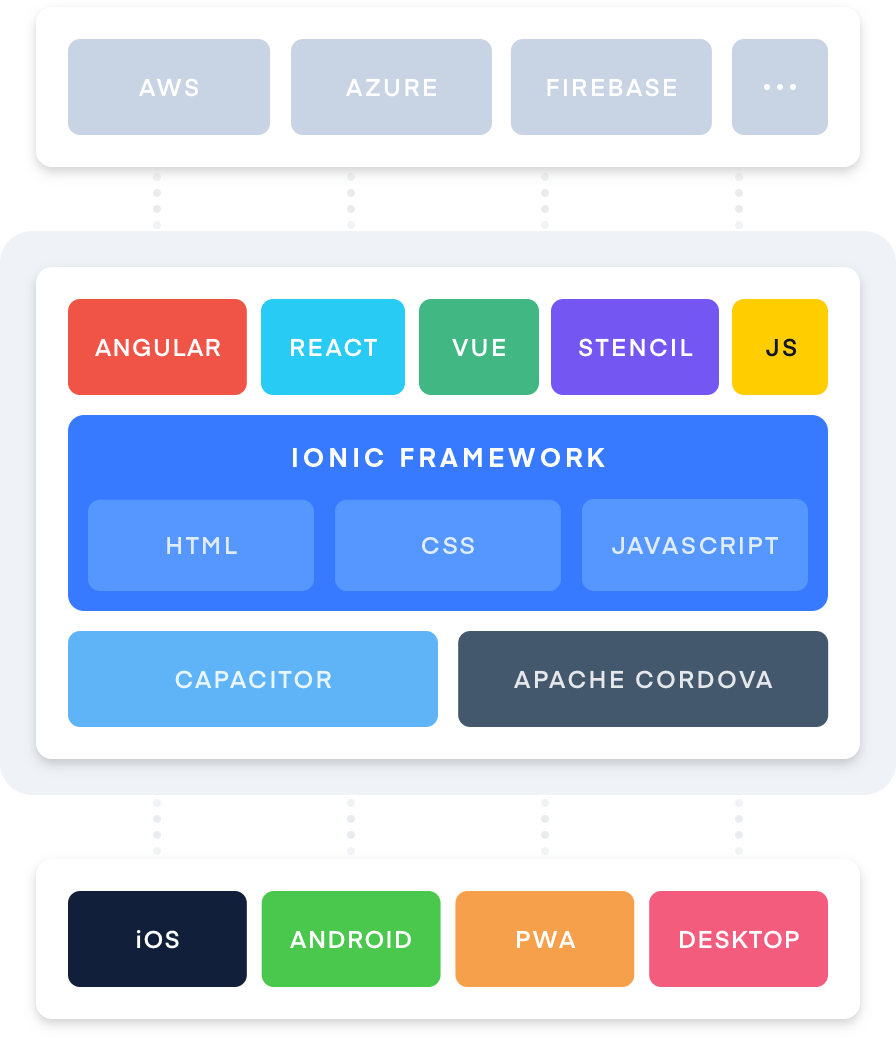
\includegraphics[width=0.72\textwidth]{ionic_architecture.png}
    \caption{Architektur des Ionic-Frameworks \cite{Ionic_Architektur}}
    \label{fig:ionic_architecture}
\end{figure}
Ionic stellt vor allem UI-Komponenten zur Verfügung, die plattformübergreifend genutzt werden können und automatisch dem Stil der jeweiligen Plattform angepasst werden.
Zur weiteren Vereinfachung bietet Ionic die Unterstützung der beliebten Frontend-Frameworks und Bibliotheken Angular, React und Vue.js.
Eine Ionic-Anwendung lässt sich auch mit anderen Frontend-Technologien oder komplett ohne Frontend-Framework erstellen \cite{Ionic_Docs, Ionic_EvaluationGuide}.
Zusätzlich erleichtert Ionic die Nutzung von TypeScript als Ersatz für JavaScript und bietet dafür typsichere Versionen von einigen Open-Source Plugins an. %TODO beleg
Ein weiterer Grund, der insbesondere Firmenkunden anspricht, sind die angebotenen Zusatzleistungen.
Für zahlende Kunden bietet Ionic persönliche Beratung und Support, ein eigenes \ac{CD} System und proprietäre Plugins für verschiedene Funktionen, die nicht über Open-Source Plugins abgedeckt werden können \cite{Ionic_EvaluationGuide}.


\subsection{Apache Cordova und Capacitor}
\label{sec:Cordova_Capacitor}
Die beiden unterstützen Cross-Plattform Frameworks Cordova und Capacitor sind sich im Allgemeinen sehr ähnlich.
Beide ermöglichen es, Webanwendungen in native Anwendungen einzubetten und über ein Plugin-System auf native \acp{API} zuzugreifen \cite{Ionic_Cordova_vs_Capacitor}.


Apache Cordova ist das deutlich ältere Framework und wird als Open-Source-Projekt von der Apache Software Foundation verwaltet.
Ursprünglich wurde Cordova von Nitobi, einer später von Adobe aufgekauften Firma, als kommerzielles Produkt entwickelt.
Eine Open-Source Version wurde 2011 an die Apache Software Foundation übergeben \cite{Steyer_Cordova}.
Die kommerzielle Version des Frameworks wurde bis 2020 von Adobe als \textit{Adobe PhoneGap} vertrieben \cite{Adobe_PhoneGap_EOL}.
Aufgrund ihrer großen Ähnlichkeit wird in der Literatur meist nicht zwischen Adobe PhoneGap und der Open-Source Variante Apache Cordova unterschieden und beide Bezeichnungen werden teilweise synonym verwendet \cite{Steyer_Cordova,Manchanda_CrossPlatformFrameworks,Rieger_CrossPlatform_EvaluationFramework}. %TODO eventuell raus

Zur Unterstützung mehrerer Plattformen verwendet Cordova den Ansatz einer Hybrid Web App.
Jede Web-App, welche komplett mit \ac{HTML}, \ac{CSS} und JavaScript entwickelt wurde, lässt sich mit Cordova als native Anwendung verpacken.
\autoref{fig:cordova_architecture} zeigt die Architektur, die sich durch die Einbettung einer Web-App in einer nativen App ergibt.
\begin{figure}[h]
    \centering
    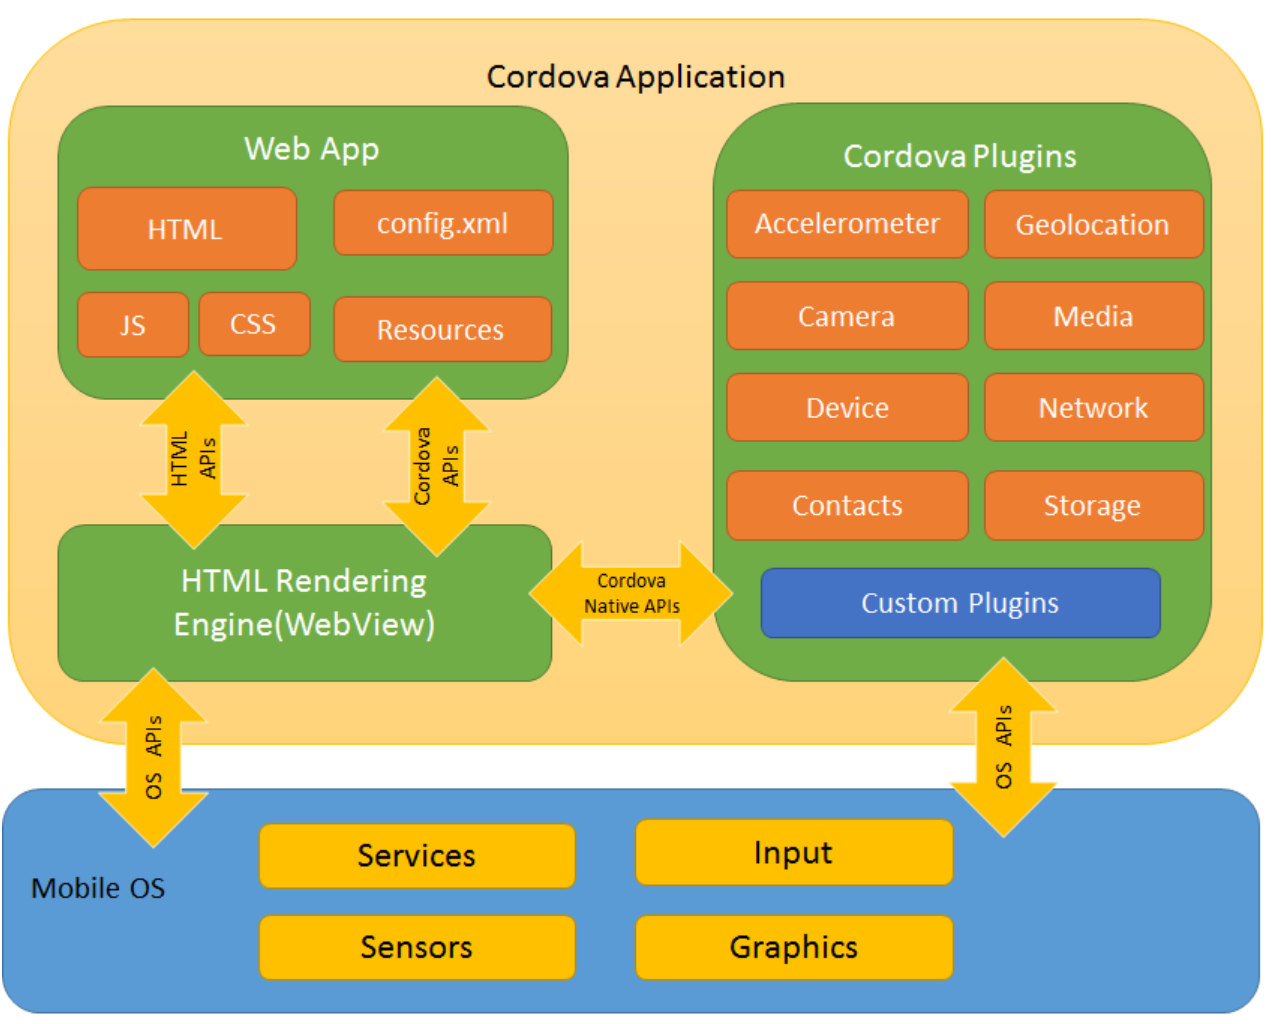
\includegraphics[width=0.85\textwidth]{cordova_architecture.png}
    \caption{Überblick über die Architektur einer Cordova-Anwendung \cite{Cordova_Overview}.}
    \label{fig:cordova_architecture}
\end{figure}



Theoretisch sind Web-Apps auch ohne den Einsatz von Cordova bereits plattformunabhängig, da sie auf verschiedenen Plattformen im Browser ausgeführt werden können.
Mit Cordova kann auf den Umweg über den Browser verzichtet werden und die Anwendung lässt sich über den App-Store der jeweiligen Plattform verbreiten.
Dazu verwendet Cordova eine Wrapper-Anwendung, welche die eigentliche Web-App in einer WebView ausführt.
Die WebView ist ein eingebetteter Webbrowser, der vom Betriebssystem bereitgestellt wird \cite{Steyer_Cordova}.
Zusätzlich können Cordova-basierte Anwendungen das bereits erwähnte und Plugin-System nutzen, um auf native Funktionen zuzugreifen \cite{Heitkoetter_CrossPlatform_Comparison}.
Der Zugriff auf native \acp{API} durch Plugins wird auch in \autoref{fig:cordova_architecture} verdeutlicht.
Für häufig verwendete Gerätefunktionen und \acp{API} stellt die Apache Software Foundation einige offizielle Plugins zur Verfügung.
Für eine Vielzahl von weiteren Funktionen sind Open-Source Plugins von anderen Anbietern verfügbar. 
Darüber hinaus erlaubt das Framework die Entwicklung eigener Plugins \cite{Cordova_Overview}.

Ein Plugin ist dabei eine JavaScript-Schnittstelle zu nativem, plattformspezifischem Code.
Aufrufe der Funktionen eines Plugins werden in der WebView zu Aufrufen der nativen Implementierung aufgelöst.
Der native Code muss die JavaScript-Schnittstelle implementieren, ist aber ansonsten in keiner Weise limitiert und kann alle verfügbaren \acp{API} verwenden.
Damit lassen sich alle Gerätefunktionen uneingeschränkt nutzen und bei Bedarf lässt sich die Performance von kritischer Funktionalität durch die Auslagerung in ein Plugin steigern.
Allerdings muss die Plugin-Funktionalität für jede zu unterstützende Zielplattform neu implementiert werden \cite{Steyer_Cordova}.
Werden ausschließlich Open-Source Plugins oder zugekaufte Plugins verwendet, kann der komplette Code der Anwendungen sowohl für Android als auch für iOS zum Einsatz kommen.
Allerdings sind einige Plugins nicht für alle Plattformen verfügbar oder funktionieren nicht auf allen Plattformen gleichermaßen \cite{Cordova_Plugin_Problem}.
Werden Funktionen benötigt, für die keine Plugins verfügbar sind, müssen eigene Plugins entwickelt werden.
Damit steigt der Entwicklungsaufwand enorm, was den Vorteil der Widerverwendung von Code schmälert.
Damit der große Vorteil der Cross-Plattform Entwicklung erhalten bleibt, sollten so wenige spezifische Plugins entwickelt werden müssen wie möglich \cite{Cordova_Development_Tips}.


Capacitor wurde 2018 von Ionic als modernere Alternative zu Cordova vorgestellt.
Wie Cordova, setzt Capacitor auf die Ausführung von Web-Apps in einer WebView innerhalb einer plattformspezifischen Wrapper-App.
Das Framework soll einige Schwachstellen von Cordova beheben und ist bei neuen Ionic-basierten Projekten die empfohlene Alternative zu Cordova.
Um den Umstieg von Cordova auf Capacitor zu erleichtern, können alle Cordova-Plugins direkt in Capacitor-Projekte eingebunden werden.
Für viele häufig verwendete Funktionen, stellt Ionic eigene Plugins für Capacitor zur Verfügung, deren Wartung und Support das Unternehmen übernimmt.
Zudem erlaubt Capacitor durch ein geändertes Build-Konzept eine einfachere Integration von nativem Code, ohne den Einsatz von Plugins \cite{Ionic_Cordova_vs_Capacitor}.
In Cordova-Projekten werden die nativen Projekte für die Wrapper-Anwendungen beim Build erzeugt und der Web-Code in diese eingebettet.
Bei Capacitor-Projekten werden die nativen Projekte für die Wrapper-Anwendungen bereits zu Beginn erstellt und sollen in die Versionsverwaltung aufgenommen werden.
Dadurch kann nativer Code direkt in die jeweiligen nativen Projekte integriert werden und wird nicht beim nächsten Build überschrieben.
Allerdings wird der Verwaltungsaufwand durch die separaten Projekte für die Wrapper-Anwendungen erhöht \cite{Liebel_Cordova_Capacitor}.


Die Performance von Ionic und Cordova-basierten Anwendungen gilt allgemein als niedrig.
Bei reinen Cordova-Anwendungen wird zusätzlich die Konsistenz der \ac{UI} häufig kritisiert.
Beides ist auf die Einbettung von Web-Apps in native Wrapper-Anwendungen zurückzuführen.
Durch die Interpretation von JavaScript-Code innerhalb der WebView und den aufwändigen Zugriff auf native Funktionen über das komplexe Plugin-System, liegt die Performance von Cordova-Anwendungen deutlich unter der von nativen Anwendungen und häufig auch unter der von anderen Frameworks \cite{Rieger_CrossPlatform_EvaluationFramework,Manchanda_CrossPlatformFrameworks,Heitkoetter_CrossPlatform_Comparison,Biorn-Hansen_PerformanceOverhead_CrossPlatform}.


Capacitor ist trotz geringerer Verbreitung deutlich beliebter als Cordova \cite{Stackoverflow_2022,Appfigures_TopSDKs}.
Von allen Entwicklern, die bereits mit Capacitor gearbeitet haben, geben 62,35 \% an, das Framework auch weiterhin einsetzen zu wollen.
Nur 28,85 \% wollen Cordova weiter verwenden.
Damit schneidet Cordova von allen betrachteten Cross-Plattform Frameworks am schlechtesten ab.
\subsection{Xamarin}
\label{sec:frameworks_xamarin}

Das von Microsoft entwickelte Xamarin-Framework ermöglicht die plattformübergreifende App-Entwicklung in C\# und dem .NET Framework und besteht seit 2011.
Neben Android und iOS werden auch Windows und macOS unterstützt.
Laut Microsoft können „bis zu 90 \% des Codes“ \cite{Xamarin_Homepage} wiederverwendet werden.
Dazu werden häufig verwendete Funktionen über abstrahierte Schnittstellen bereitgestellt und für \acp{API} der Plattformen existieren Bindings in C\#, sodass diese direkt aufgerufen werden können.
Außerdem können native Bibliotheken eingebunden werden, sodass beliebiger Code in der jeweiligen plattformspezifischen Sprache integriert werden kann \cite{Xamarin_Android}.


Zur Ausführung von .NET-Code auf den mobilen Plattformen, wird die Mono-Ausführungsumgebung verwendet, eine Open-Source Runtime für .NET.
Parallel kommt jeweils eine native Ausführungsumgebung zum Einsatz, welche den Aufruf von Plattform-\acp{API} und die Interoperabilität mit nativem Code ermöglicht.
Unter Android wird hierfür die \ac{ART} verwendet, unter iOS die Objective-C Ausführungsumgebung \cite{Xamarin_iOS,Xamarin_Android}.
Die sich ergebende Architektur ist in \autoref{fig:xamarin_architecture} dargestellt.
Die in C\# bereitgestellten Bindings zu nativen Funktionen werden von der Ausführungsumgebung in die passenden nativen Aufrufe übersetzt.
\begin{figure}[h]
    \centering
    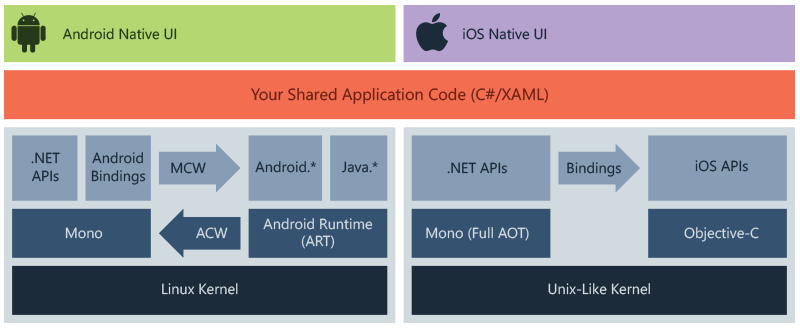
\includegraphics[width=0.95\textwidth]{xamarin_architecture.png}
    \caption{Architektur einer Xamarin-App \cite{Xamarin_Homepage}.}
    \label{fig:xamarin_architecture}
\end{figure}


Durch die Verwendung von C\# ist Xamarin nach Nunkessers Taxonomie \cite{Nunkesser_Taxonomy_Apps} eine Foreign Language App.
Um die Verwendung von C\# unter Android und iOS zu ermöglichen, wird der Code zunächst mithilfe des Mono-Compilers in das Zwischencodeformat \ac{MSIL} kompiliert.
Normalerweise wird dieser Code beim Anwendungsstart von der .NET \ac{CLR} mit einem \ac{JIT}-Compiler zu Plattformspezifischem Code kompiliert.
Für iOS-Anwendungen wird der \ac{MSIL}-Code jedoch \ac{AOT} kompiliert, da Apple unter iOS die Ausführung von dynamisch erzeugtem Code aus Sicherheitsgründen nicht erlaubt \cite{Xamarin_iOS}.
Der Buildprozess einer Xamarin-Anwendung mit den beiden Zielplattformen Android und iOS ist in \autoref{fig:xamarin_build} dargestellt.
\begin{figure}[h]
    \centering
    
\includegraphics[clip, trim=3cm 20cm 2cm 0, width=0.9\textwidth]{xamarin_build.pdf}
    \caption{Buildprozess einer Xamarin-Anwendung für die Plattformen Android und iOS.}
    \label{fig:xamarin_build}
\end{figure}


Ein großes Problem von Xamarin besteht darin, dass typischerweise für jede Plattform eine eigene native Benutzerschnittstelle entwickelt werden muss, wie auch in \autoref{fig:xamarin_architecture} gezeigt \cite{Xamarin_Homepage}.
Das erhöht den Aufwand im Vergleich zu anderen Frameworks, welche standardmäßig eine plattformübergreifende Benutzerschnittstelle bereitstellen.
Deshalb bietet Xamarin mit der \ac{UI}-Bibliothek Xamarin.Forms eine Erweiterung zur plattformübergreifenden Entwicklung von Oberflächen \cite{Xamarin_Homepage}.
Auf der Konferenz Microsoft Build, hat das Unternehmen 2020 angekündigt das Xamarin-Framework besser in .NET zu integrieren und im Zusammenhang die Bezeichnung Xamarin abzuschaffen.
Stattdessen werden die Komponenten Xamarin.Android und Xamarin.iOS in \textit{.NET for Android} und \textit{.NET for iOS} umbenannt, wobei die zugrundeliegende Technologie erhalten bleibt \cite{MS_Build_2020}.
Xamarin fließt damit komplett in .NET ein und ist nicht mehr als eigenständiges Framework zu betrachten.
Der Support für Xamarin endet am ersten Mai 2024 \cite{Xamarin_EOL}.
Als Nachfolger für Xamarin wurde auf der Microsoft Build 2020 das Framework .NET \ac{MAUI} angekündigt.
Der Namen verdeutlicht einen starken Fokus auf plattformübergreifende Entwicklung von Benutzerschnittstellen, weshalb .NET \ac{MAUI} auch als Weiterentwicklung von Xamarin.Forms angesehen wird \cite{NET_MAUI_Introduction}.
Allerdings übernimmt das Framework auch die Abstraktion der verschiedenen .NET Implementierungen auf den einzelnen Zielplattformen und wird von Microsoft explizit als Cross-Plattform Framework beworben \cite{NET_MAUI}.
Technisch kann .NET \ac{MAUI} daher als Weiterentwicklung von Xamarin insgesamt betrachtet werden und beide Bezeichnungen werden aktuell teilweise noch synonym verwendet.
Da die erste Version von .NET \ac{MAUI} erst im Mai 2022 veröffentlicht wurde \cite{NET_MAUI_Release}, wird in dieser Arbeit weiterhin von Xamarin gesprochen.


Xamarin-Anwendungen weisen allgemein eine durchschnittliche Performance im Vergleich zu anderen Frameworks auf \cite{Nawrocki_Comparison_Hybrid_Native_Frameworks, Bakker_Xamarin_XamarinForms_Native, Xamarin_Homepage}.
Durch die \ac{JIT}-Kompilierung und Android kann die Startzeit jedoch vergleichsweise lang ausfallen \cite{Nawrocki_Comparison_Hybrid_Native_Frameworks}.
Unter iOS ist dieser Nachteil nicht gegeben, allerdings sind dafür die Apps um einiges größer als nativ entwickelte Apps.
Nawrocki \textit{et al.} \cite{Nawrocki_Comparison_Hybrid_Native_Frameworks} berichten von einem bis zu 16-fachen Speicherbedarf.

In der Stackoverflow-Umfrage 2022 \cite{Stackoverflow_2022} gibt eine Mehrheit von 61,47 \% der Entwickler, die bereits mit Xamarin gearbeitet haben, an, das Framework nicht weiterhin verwenden zu wollen.
Bis auf Cordova schneiden alle anderen, in dieser Arbeit untersuchten Cross-Plattform Frameworks besser ab.
Inwiefern die Beliebtheit auf Probleme bei der Benutzung oder beim Zugriff auf Gerätefunktionen zurückzuführen ist, wird sich im Laufe dieser Arbeit zeigen.
\section{ReactNative}
\label{sec:Frameorks_ReactNative}

Das von Meta, ehemals Facebook, entwickelte ReactNative Framework ermöglicht die Cross-Plattform Entwicklung mit Webtechnologien.
Dabei kommt die verbreitete \ac{UI}-Bibliothek React zum Einsatz, um die Benutzeroberfläche zu erstellen.
Als Zielplattformen werden neben Android und iOS unter anderem Windows und macOS unterstützt \cite{ReactNative}.
Ein großer Vorteil des Frameworks ist die Verwendung von React für die Umsetzung der \ac{UI}.
Da viele Webentwickler mit React vertraut sind, fällt die Einarbeitung in ReactNative leicht, was zu einer großen Verbreitung des Frameworks führt \cite{Appfigures_TopSDKs,Stackoverflow_2022}.
Außerdem lässt sich ReactNative vergleichsweise einfach in bestehende native Projekte integrieren, was die inkrementelle Migration von Projekten ermöglicht.
Diese Integrationsmöglichkeit führt auch dazu, dass neben den Apps von Meta, weitere populäre Apps wie die Microsoft Office Apps, Pinterest und WordPress teile ihrer Funktionalität mit ReactNative umsetzen \cite{ReactNative_Showcase}.


Obwohl ReactNative wie Cordova und Capacitor auf Webtechnologien, insbesondere JavaScript, basiert, wählt das Framework einen anderen Ansatz, um die Cross-Plattform Entwicklung zu ermöglichen.
Mit Ionic können Cordova und Capacitor Apps ebenfalls React als \ac{UI}-Bibliothek verwenden.
Dabei ist die Oberfläche komplett als Webanwendung implementiert und wird in einer WebView der jeweiligen Plattform dargestellt.
ReactNative verzichtet hingegen auf den Einsatz einer WebView und nutzt stattdessen die nativen \ac{UI}-Komponenten der jeweiligen Plattformen.
Der JavaScript Code wird nicht, wie bei Foreign Language Apps nach Nunkesser \cite{Nunkesser_Taxonomy_Apps}, in nativ ausführbaren Code übersetzt, sondern in einer JavaScript-Runtime ausgeführt.
Somit lässt sich ReactNative weder komplett den Hybrid Web Apps noch den Foreign Language Apps zuordnen.
Stattdessen handelt es sich um Hybrid Bridged Apps, da Webtechnologien und native \ac{UI}-Elemente in einer App kombiniert werden.


Aktuell wird die Architektur von ReactNative auf einen neuen Ansatz umgestellt, der Probleme der bisherigen Architektur beheben soll.
Da jedoch noch beide Ansätze unterstützt werden, wird hier sowohl auf die bisherige als auch auf die neue Architektur eingegangen.

Die bisherige Architektur setzt sich aus zwei Komponenten zusammen, welche über die sogenannte ReactNative Bridge miteinander kommunizieren.
Die Bridge trennt dabei den JavaScript Code von der nativen Umgebung.
Der JavaScript-Code wird in einem eigenen Thread innerhalb der JavaScriptCore Ausführungsumgebung, einem Teil der Open-Source Browser Engine WebKit, ausgeführt.
Dieser Thread wird auch als JavaScript-Thread oder kurze JS-Thread bezeichnet.
Unter iOS ist die WebKit Engine die einzige erlaubte Browser Engine und dementsprechend standardmäßig auf allen iOS Geräten installiert und kann von ReactNative-Apps genutzt werden.
Android liefert die JavaScriptCore nicht mit, weshalb ReactNative-Apps für Android JavaScriptCore mitliefern müssen und demnach größer ausfallen \cite{Dragomir_ReactNative,Nawrocki_Comparison_Hybrid_Native_Frameworks}.
Die \ac{UI} wird von der nativen Umgebung, dem sogenannten nativen Thread, gerendert.
Die Bridge übernimmt im Wesentlichen die Kommunikation zwischen den beiden Thread.
Render-Anweisungen werden vom JS-Thread an den nativen Thread gesendet und umgekehrt werden Eingaben und Events vom nativen Thread an den JS-Thread übermittelt.
Die Kommunikation erfolgt über Nachrichten, welche im \ac{JSON} Format serialisiert übertragen werden \cite{Dragomir_ReactNative}.

% TODO: Performance problem dieser architektur und Weg zur neuen -> \cite{Cook_ReactNativeBridge}



%TODO: Architektur


%TODO: Beliebtheit, mögliche Performanceprobleme
